
\subsection{Library Design}

TUG Base Library is the supporting library used by test projects
generated using TUG Wizard. Its architecture design is depicted in the
figure below. 

\vspace{2ex}
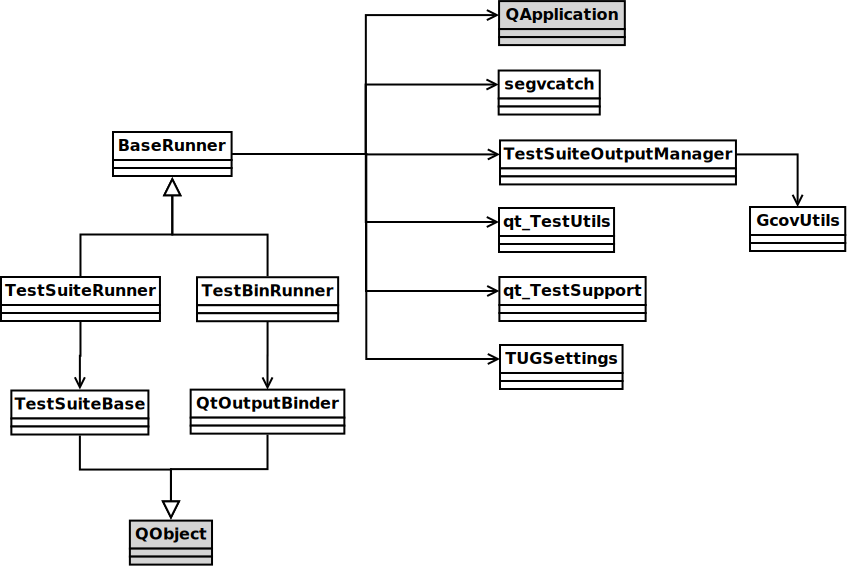
\includegraphics[width=.99\textwidth]{images/diag/tug_lib_classdiag.png}
\vspace{2ex}

Main elements of this architecture are described in the following:
\begin{itemize}
\item {\tt TestSuiteBase}
\item {\tt BaseRunner}
\item {\tt TestSuiteRunner}
\item {\tt TestBinRunner}
\item {\tt qt\_TestUtils}
\item {\tt qt\_TestSupport}
\end{itemize}

\newpage

%%%
%%%
\field{TestSuiteBase} is the base class for any testsuite. It
implements the basic functionality of a test suite, and includes also
some virtual methods to be implemented in subclasses. It extends {\tt
  QObject} class to be integrated in Qt Test framework.


The code snippet below shows how new testsuites have to be defined:

\begin{lstlisting}
#include "TestSuiteBase.h"

class Testsuite_base_Panel : public TestSuiteBase {

    Q_OBJECT /// Our test suite has to execute Q_OBJECT macros

    (...)
\end{lstlisting}

Testsuites based on {\tt TestSuiteBase} can be created as object and
executed standalone by using the following methods:

\begin{lstlisting}
//
static int 
 launch_standalone (TestSuiteBase* tsb, int argc=0, char *argv[]=0);
//
static int 
 launch (TestSuiteBase* tsb, QApplication* app);
//
static int 
 launch (TestSuiteBase* tsb, QApplication* app, int argc,char** argv);
\end{lstlisting}


One or more {\tt TestSuiteBase} objects can be also be launched
sequentially using {\tt TestSuiteRunner}, as described below.


\newpage

%%%
%%%
\field{BaseRunner} includes the basic functionality to run tests. Tests
can be run from a testsuite class file using {\tt TestSuiteRunner}, or
from a testsuite binary using {\tt TestBinRunner}. 
%
The former has the advantage that no previously compiled binaries are
needed, and that all tests are encapsulated into a single binary file.
%
The latter has the advantage that tests are executed as independent
binary files, allowing thus to handle segmentation faults. This is the
option used in TUG Wizard.

All relevant methods and options supported by {\tt BaseRunner} are
described in the following:
\begin{itemize}
%
\item {\tt BaseRunner\& add\_timestamp\_to\_output\_filename()}: adds a
  timestamp to the name of the generated output files.
%
\item {\tt BaseRunner\& coverage\_on\_dir(const std::string\& dir)}:
  includes directory {\tt dir} into coverage analysis.
%
\item {\tt BaseRunner\& coverage\_on\_file(const std::string\&
  filepath)}: includes file {\tt filepath} into coverage analysis.
%
\item {\tt BaseRunner\& output\_***()}: selects output level between
  {\tt silent}, {\tt verbose}, {\tt extended} or {\tt all}.
%
\item {\tt BaseRunner\& pause\_between(int ms)}: sets idle time
  between the execution of a test and the following one.
%
\item {\tt BaseRunner\& project\_name(const std::string name)}: sets a
  name for the test project. This name is used if a report is
  generated.
%
\item {\tt void reset()}: resets runner values.
%
\item {\tt int run()}: run the tests previously added to the runner.
%
\end{itemize}


\newpage

%%%
%%%
\field{TestSuiteRunner} can be used to run testsuite files. It
provides the method {\tt add\_testsuite()} to add a new testsuite
object to the runner. Testsuites objects are run sequentially. If a
test causes segmentation fault or another similar error, next text
will not be executed.

The code snippet below shows how {\tt TestSuiteRunner} has to be
defined and properly configured. In the example, a project name is
given, output is configured, and coverage targets are set. A new
testsuite object is created and added to the runner. Finally, the
tests are run. 

\begin{lstlisting}
#include <TestSuiteRunner.h>
#include "testsuite_Panel_1.hpp"

int main(int argc, char *argv[])
{
    /// 1. create a TestSuiteRunner and configure...
    TestSuiteRunner trunner(argc,argv);
    trunner.project_name("PanelTestproject");

    // output options
    trunner.output_verbose();

    // coverage options
    trunner.coverage_on_file("/adir/afile.cpp")
           .coverage_on_dir("/adir/");

    /// 2. add testsuites to the runner
    testsuite_Panel_1 ts1;
    trunner.add_testsuite(&ts1);

    /// 3. run testsuites
    return trunner.pause_between(1000).run_testsuites();
}
\end{lstlisting}



\newpage


%%%
%%%
\field{TestBinRunner} can be used to run testsuite binaries (i.e.,
testsuite projects already compiled). It provides the method {\tt
  add\_testbin()} to add a new testsuite binary to the
runner. Testsuites binaries are run sequentially. If a test causes
segmentation fault or another similar error, runner tries to recover
output data and then executes next test.

The code snippet below shows how {\tt TestBinRunner} has to be defined
and properly configured. In the example, a project name is given,
output is configured, and coverage targets are set. A new testsuite
binary is added to the runner using a relative path. Finally, the
tests are run.


\begin{lstlisting}
#include <TestBinRunner.h>

int main(int argc, char *argv[])
{
    /// 1. create a test runner and configure...
    TestBinRunner trunner(argc,argv);
    trunner.project_name("PanelTestproject");

    // output options
    trunner.output_verbose();

    // coverage options
    trunner.coverage_on_file("/adir/afile.cpp")
           .coverage_on_dir("/adir/");

    /// 2. add test binaries to the runner
    trunner.add_testbin("./Testsuite_PlotCenterPanel_1_1");

    /// 3. run tests
    return trunner.pause_between(1000).run();
}
\end{lstlisting}

\vspace{2ex}


%%%
%%%
\field{qt\_TestUtils} includes a set of methods aimed at supporting the
definition of new tests (e.g., launch or repaint a panel, sleep some
milliseconds, assert values, generate random variables, simulate
segmentation faults, send data to logs, range macros, etc).\\
%
\indent \field{qt\_TestSupport} includes a set of methods to manipulate Qt GUI
widgets. These methods try to simulate user interaction.\\
%
Relevant methods in these classes are further described in next subsection.



\newpage




%%% Local variables:
%%% mode: latex
%%% TeX-master: "README.tex"
%%% ispell-local-dictionary: "american"
%%% coding: utf-8
%%% fill-column: 75
%%% TeX-parse-self: t
%%% TeX-auto-save: t
%%% End:
